\section{Phân tích và thiết kế hệ thống}
\subsection{Phân tích yêu cầu}
\subsubsection{Yêu cầu chức năng}

\textbf{Về mặt thiết bị IoT:}
\begin{itemize}
    \item [--] Cung cấp báo cáo khí hậu trực tiếp dưới dạng biểu đồ và nhật ký, giúp theo dõi nhiệt độ, độ ẩm và ánh sáng trong nhà kính.  
    \item [--] Tưới nước tự động theo độ ẩm đất và loại cây, đảm bảo cây phát triển khỏe mạnh mà không cần tưới thủ công thường xuyên.  
    \item [--] Duy trì điều kiện khí hậu lý tưởng (nhiệt độ, thông gió, chiếu sáng) bằng phương thức thủ công, tự động hoặc theo lịch trình cài đặt trước.  
    \item [--] Phát hiện và báo cáo các sự cố khi không thể duy trì điều kiện môi trường trong ngưỡng cho phép, giúp người dùng can thiệp kịp thời.  
    \item [--] Nhắc nhở định kỳ các công việc bảo trì thủ công như kiểm tra nguồn nước, vệ sinh cửa sổ và đảm bảo hệ thống thông gió hoạt động hiệu quả.
\end{itemize}

\textbf{Về mặt Web App:}
\begin{itemize}
    \item [--] Cho phép người dùng điều khiển thủ công các chức năng cụ thể trong nhà kính, như tưới cây, bật/tắt đèn và kích hoạt hệ thống cảnh báo, giúp linh hoạt trong việc quản lý môi trường trồng trọt.
    \item [--] Cung cấp số liệu khí hậu hiện tại cùng với dữ liệu lịch sử, giúp người dùng theo dõi sự thay đổi môi trường và đưa ra quyết định phù hợp cho cây trồng.
    \item [--] Thực hiện phân tích thống kê và cung cấp báo cáo chi tiết về tình trạng và hiệu suất hoạt động của hệ thống, giúp tối ưu hóa quá trình vận hành và bảo trì. 
\end{itemize}

\subsubsection{Yêu cầu phi chức năng}

\textbf{Về mặt thiết bị IoT:}
\begin{itemize}
    \item [--] Hệ thống phải hoạt động liên tục 24/7 với thời gian gián đoạn theo lịch trình không quá 2 giờ mỗi tháng và không có gián đoạn đột xuất quá 10 phút.
    \item [--] Độ trễ của bộ truyền động khi thực hiện lệnh không được vượt quá 5 giây trong 95\% trường hợp kiểm tra.
    \item [--] Hệ thống phải ghi nhật ký dữ liệu lịch sử liên tục, lưu trữ ít nhất 180 ngày với độ chính xác $\pm 1\%$ và không mất dữ liệu quá 0,1\% trong quá trình vận hành.
    \item [--] Cơ sở dữ liệu phải hỗ trợ lưu trữ tối thiểu 500MB và có thể mở rộng lên đến 2GB mà không ảnh hưởng đến hiệu suất truy xuất dữ liệu (tốc độ phản hồi dưới 1 giây cho 95\% truy vấn).
    \item [--] Hướng dẫn sử dụng phải dễ hiểu, cho phép người dùng mới vận hành hệ thống trong vòng 10 phút mà không cần trợ giúp. Giao diện LCD và nút bấm phải phản hồi trong vòng 1 giây sau khi thao tác.
\end{itemize}

\textbf{Về mặt Web App:}
\begin{itemize}
    \item [--] Hệ thống phải dễ sử dụng cho mọi độ tuổi, đặc biệt hướng đến nông dân, người làm vườn và quản lý nông nghiệp, với thời gian đào tạo không quá 15 phút.
    \item [--] Ứng dụng web phải tương thích với các trình duyệt phổ biến, bao gồm Chrome, Firefox, Edge và Safari, với hiệu suất ổn định trên cả máy tính và thiết bị di động.
    \item [--] Kết nối với máy chủ phải hoàn tất trong vòng 2 giây, trong khi các thao tác giao diện cơ bản (bấm nút, cuộn trang) phải phản hồi trong vòng 500ms.
    \item [--] Hỗ trợ lưu trữ dữ liệu cục bộ tối đa 100MB, đồng thời đồng bộ dữ liệu với máy chủ mà không làm gián đoạn hoạt động của ứng dụng.
    \item [--] Người dùng phải có thể xác thực bằng mật khẩu và/hoặc hình vẽ mẫu, với mật khẩu được lưu trữ an toàn theo tiêu chuẩn mã hóa SHA-256 hoặc cao hơn.
\end{itemize}

\subsection{Use Case Diagram}
\subsubsection{Toàn bộ hệ thống}
\begin{figure}[H]
    \centering
    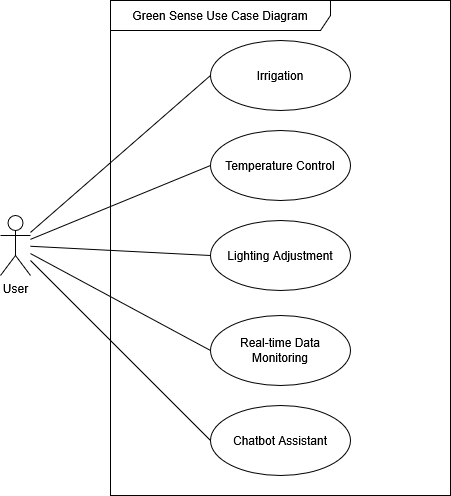
\includegraphics[width=0.5\linewidth]{content/images/GreenSense_UC_Diagram.png}
    \caption{Biểu đồ use case cho hệ thống Green Sense}
    \label{fig:useCaseDiagram}
\end{figure}
\subsubsection{Bảng mô tả cho từng use case}
\textbf{Use case 1 - Tưới nước}

\renewcommand{\arraystretch}{1.6}
\begin{table}[H]
\centering
\begin{tabular}{|p{0.2\linewidth}|p{0.7\linewidth}|}
\hline
\rowcolor[HTML]{EFEFEF} 
\textbf{Usecase}        & \textbf{Tưới nước} \\ \hline
Use case ID             & 1 \\ \hline
Actor                   & Người dùng của hệ thống \\ \hline
Description             & 
Hệ thống cung cấp ba chế độ tưới:
\begin{itemize}
    \item [--] Tự động: Duy trì độ ẩm đất theo mức cài đặt sẵn.
    \item [--] Lập lịch: Tưới theo lịch do người dùng đặt.
    \item [--] Thủ công: Người dùng tự bật/tắt tưới.
\end{itemize}
\\ \hline
Precondition            & Hệ thống đang hoạt động bình thường và được trang bị ít nhất một máy bơm, một cảm biến độ ẩm đất và một nguồn nước \\ \hline
Postcondition           & Dữ liệu độ ẩm đất được ghi lại theo tần suất mà kế hoạch hiện tại kiểm tra độ ẩm. Ngoài ra, hệ thống cũng lưu trữ nhật ký tất cả các lần tưới, kèm theo thông tin về sự kiện kích hoạt tưới. \\ \hline
Normal Flow             & 
Quy trình hoạt động dự kiến là người dùng ủy quyền việc tưới tiêu cho hệ thống.\newline
1. Người dùng mở trang web của hệ thống. \newline
3. Người dùng chọn "Tưới tiêu" từ danh sách tính năng trên giao diện chính. \newline
4. Người dùng chọn "Tự động" trong phần Chế độ. \newline
5. Người dùng đặt mức độ ẩm mục tiêu theo bảng giá trị khuyến nghị trên màn hình hoặc điều chỉnh bằng thanh trượt để chọn giá trị tùy chỉnh. \newline
6. Hệ thống đánh giá từng phép đo nhận được và thực hiện hành động nếu cần. Cụ thể, nếu độ ẩm thấp hơn 50\% so với mức mục tiêu, hệ thống sẽ tưới trong 5 giây. 
\\ \hline
Alternative Flow          & 
    Tại bước 4, nếu người dùng chọn tưới theo lịch: \newline
    4.1 Người dùng chọn thêm một nhiệm vụ tưới mới. \newline
    4.2 Người dùng chọn khoảng thời gian lập lịch (theo chế độ Cron hoặc chế độ Interval). Biểu mẫu tương ứng sẽ hiển thị. \newline
    4.3 Người dùng đặt thời gian tưới trong lịch trình đó và đặt thời gian bơm nước cần sử dụng. \newline
    4.4 Hệ thống tưới theo lịch trình đã đặt. Nếu hành động tự động được bật, hệ thống sẽ theo dõi độ ẩm đất mỗi khi có dữ liệu mới và có thể gửi cảnh báo qua thông báo nếu cần. \newline
    Tại bước 4, nếu người dùng chọn tưới hoàn toàn thủ công:\newline
    4.1 Người dùng chỉ định hệ thống bật bơm nước trong khoảng thời gian do người dùng tự thiết lập
    Chi tiết về giao diện ứng dụng có thể thay đổi trong quá trình phát triển.
 \\ \hline
\end{tabular}
\end{table}

\begin{table}[H]
\begin{tabular}{|p{0.2\linewidth}|p{0.7\linewidth}|}
    \hline
    Exception Flow          & 
        Tại bước 6, nếu hệ thống phát hiện sự thay đổi bất thường (hoặc không có thay đổi) trong độ ẩm đất khi đang tưới: \newline
        a. Hệ thống không phát hiện sự thay đổi độ ẩm nhanh như mong đợi hoặc không có thay đổi nào. \newline
        b. Hệ thống gửi thông báo đẩy đến ứng dụng trên điện thoại, cảnh báo về sự cố với nguồn nước (hết nước hoặc tắc nghẽn) hoặc bơm. \newline
        c. Nếu cơ chế dự phòng được kích hoạt, hệ thống thực hiện hành động mạnh hơn (bật bơm trong 20 giây). 
    \\ \hline
    \end{tabular}
\caption{Bảng mô tả cho use case Tưới nước}
\end{table}



\textbf{Use case 2 - Điều chỉnh nhiệt độ}
\renewcommand{\arraystretch}{1.6}
\begin{table}[H]
\centering
\begin{tabular}{|p{0.2\linewidth}|p{0.7\linewidth}|}
\hline
\rowcolor[HTML]{EFEFEF} 
\textbf{Usecase}        & \textbf{Điều chỉnh nhiệt độ} \\ \hline
Use case ID             & 2 \\ \hline
Actor                   & Người dùng của hệ thống \\ \hline
Description             & 
    Với tính năng kiểm soát nhiệt độ, hệ thống cung cấp 3 lựa chọn:
    \begin{itemize}
        \item [--] \textbf{Chế độ tự động:} Hệ thống cố gắng duy trì nhiệt độ bên trong nhà kính ở mức lý tưởng.
        \item [--] \textbf{Chế độ theo lịch:} Tuân theo lịch trình mà người dùng cài đặt, kèm theo tùy chọn dự phòng an toàn (nếu muốn) để hệ thống tự điều chỉnh khi có biến động bất thường.
        \item [--] \textbf{Chế độ thủ công:} Người dùng toàn quyền điều khiển đóng/mở các tấm che nắng (là những tấm che trên trần có khả năng cản sáng; trong mô hình này, chúng ta dùng động cơ mô phỏng việc cuốn/mở tấm che), bất cứ khi nào họ muốn.
    \end{itemize}
\\ \hline
Precondition            & 
Hệ thống đang vận hành bình thường. \newline
Hệ thống được trang bị cảm biến DHT20 để đo nhiệt độ và độ ẩm. \newline
Tùy chọn, hệ thống có lắp các tấm che nắng kết nối với bộ truyền động (Động cơ Servo SG90S) để cuộn vào hoặc mở ra. 
\\ \hline
Postcondition           & 
Nhiệt độ (đo bởi cảm biến) và trạng thái của tấm che nắng được ghi nhận vào cơ sở dữ liệu của hệ thống theo định kỳ. \newline
Mọi hành động điều chỉnh nhiệt độ (do người dùng thực hiện hoặc do hệ thống tự động) đều được ghi lại vào lịch sử.
\\ \hline
Normal Flow             & 
1. Người dùng mở trang web của hệ thống. \newline
2. Người dùng chọn “Temperature control” (Kiểm soát nhiệt độ) từ danh sách tính năng trên màn hình chính. \newline
3. Người dùng chọn “Scheduled mode” (Chế độ theo lịch). \newline
4. Người dùng chọn khung giờ mong muốn và chọn góc độ để tấm che nắng mở hoặc đóng.
\\ \hline
Alternative Flow 1        & 
3.1. Tại bước 3, nếu người dùng chọn “Automatic” (Tự động): \newline
3.1.1 Người dùng chỉ định khoảng nhiệt độ mục tiêu. \newline
3.1.2 Hệ thống bắt đầu kiểm tra mức nhiệt mỗi khi có dữ liệu mới từ cảm biến. Ví dụ, nếu nhiệt độ bên trong nhà kính thấp hơn khoảng mục tiêu từ 3 đến 5 độ C, hệ thống sẽ mở các tấm che nắng theo góc mà người dùng đã cài đặt từ trước
\\ \hline
Alternative Flow 2        & 
3.2. Tại bước 3, nếu người dùng chọn “Manual” (Thủ công): \newline
3.2.1 Người dùng chỉ định góc độ mà tấm che nắng sẽ mở và chọn "điều khiển tấm che nắng" \newline
3.2.2 Tấm che nắng sẽ được mở với góc độ mà người dùng đã cài đặt
\\ \hline
\end{tabular}
\caption{Bảng mô tả cho use case Điều chỉnh nhiệt độ}
\end{table}

\textbf{Use case 3 - Điều chỉnh ánh sáng}
\renewcommand{\arraystretch}{1.6}
\begin{table}[H]
\centering
\begin{tabular}{|p{0.2\linewidth}|p{0.7\linewidth}|}
\hline
\rowcolor[HTML]{EFEFEF} 
\textbf{Usecase}        & \textbf{Điều chỉnh ánh sáng} \\ \hline
Use case ID             & 3 \\ \hline
Actor                   & Người dùng của hệ thống \\ \hline
Description             & Chúng ta có thể tùy chỉnh cho phù hợp các mức độ ánh sáng phù hợp trong nhà trồng cây với 3 chế độ: tự động điều chỉnh phù hợp với điều kiện môi trường, lập lịch các khoảng thời gian trong ngày hoặc các ngày trong tuần, hoặc người dùng có thể điều chỉnh ánh sáng của đèn trực tiếp. \\ \hline
Precondition            & Hệ thống hoạt động bình thường và luôn được trang bị cảm biến ánh sáng và một mạch role gắn vào nguồn chiếu sáng của nguồn chiếu sáng. \\ \hline
Postcondition           & Hệ thống ánh sáng hoạt động đúng như cách người dùng thiết lập. Các hành động điều chỉnh mức độ sáng bởi người dùng hay hệ thống đều được lưu vào lịch sử theo dõi. \\ \hline
Normal Flow             & 
    1. Người dùng mở trang web của hệ thống. \newline
    2. Người dùng chọn ``Điều chỉnh chế độ sáng" từ danh sách các tính năng trên màn hình chính. \newline
    3. Người dùng chọn ``Lập lịch". \newline
    4. Hệ thống cung cấp một thanh trượt dựa trên phạm vi biểu thị 24h trong ngày. \newline
    5. Người dùng chọn khoảng thời gian mong muốn trong ngày để đèn hoạt động và các mức độ để đèn bật (với cường độ sáng tăng từ 1 đến 4, tắt đèn là 0). 
\\ \hline
Alternative Flow 1          & 
    3.1. Ở bước 3, nếu người dùng chọn `Tự động' trên thanh tùy chọn: \newline
    3.1.1. Người dùng chọn cụ thể mức độ sáng mục tiêu \newline
    3.1.2. Hệ thống bắt đầu kiểm tra và nhận dữ liệu về sau mỗi đơn vị thời gian. Nếu mức độ sáng không phù hợp với cấu hình không đúng với mục tiêu, hệ thống sẽ điều chỉnh đến khi nào cảm biến ánh sáng nhận được dữ liệu với mức độ sáng theo cách người dùng thiết lập  \\ \hline
Alternative Flow 2          & 
    3.2. Ở bước 3, nếu người dùng chọn `Thủ công' trên thanh tùy chọn: \newline
    3.2.1. Người dùng thiết lập độ sáng cho đèn (với cường độ sáng tăng từ 1 đến 4, tắt đèn là 0) và chọn ``Điều khiển đèn" \newline 
    3.2.2. Đèn sẽ được bật/tắt theo thiết lập của người dùng. \\ \hline
\end{tabular}
\caption{Bảng mô tả cho use case Điều chỉnh ánh sáng}
\end{table}

\textbf{Use case 4 - Theo dõi dữ liệu theo thời gian thực và thống kê hệ thống}
\renewcommand{\arraystretch}{1.6}
\begin{table}[H]
\centering
\begin{tabular}{|p{0.2\linewidth}|p{0.7\linewidth}|}
\hline
\rowcolor[HTML]{EFEFEF} 
\textbf{Usecase}        & \textbf{Theo dõi dữ liệu theo thời gian thực và thống kê hệ thống} \\ \hline
Use case ID             & 4 \\ \hline
Actor                   & Người dùng của hệ thống \\ \hline
Description             & Ứng dụng cho phép người dùng xem dữ liệu đã ghi dưới dạng báo cáo tổng hợp (trong một khoảng thời gian) với các tính toán tổng hợp và biểu đồ tổng quan về các bản ghi trước đó. \\ \hline
Precondition            & Trang web được kết nối với cơ sở dữ liệu và hệ thống vẫn đang ghi lại thống kê. \\ \hline
Postcondition           & Không có.  \\ \hline
Normal Flow             & 
    1. Người dùng mở trang web của hệ thống. \newline
    2. Người dùng chọn `Thống kê' từ danh sách các tính năng trên màn hình chính. \newline
    3. Hệ thống trích xuất dữ liệu hàng ngày làm chế độ báo cáo mặc định và hiển thị cho người dùng. Báo cáo bao gồm biểu đồ đường về mức ánh sáng, độ ẩm và nhiệt độ trong khoảng thời gian đó; các hành động đáng chú ý được thực hiện thủ công hoặc tự động trên hệ thống nhà kính; và trạng thái mới nhất của nhà kính (các phép đo nhận được gần nhất). \newline
    4. Người dùng có thể chọn khoảng thời gian ưa thích bằng cách chọn `Khoảng thời gian' trên thanh tùy chọn. \newline
    5. Hệ thống cung cấp lịch chi tiết để người dùng chọn ngày bắt đầu và ngày kết thúc cho báo cáo. \newline
    6. Người dùng chọn khoảng thời gian ưa thích và nhấn `Xác nhận'. \newline
    7. Hệ thống tải lại trang báo cáo với chế độ hiển thị biểu đồ phù hợp và theo dõi hành động. \newline
    8. Người dùng nhấn `Hoàn tất' để quay lại trang chính.
\\ \hline
Alternative Flow          & 
\\ \hline
Exception Flow          &  
\\ \hline
\end{tabular}
\caption{Bảng mô tả cho use case Theo dõi dữ liệu theo thời gian thực và thống kê hệ thống}
\end{table}

\textbf{Use case 5 - Điều khiển IoT Device trong hệ thống bằng Chatbox AI}

\renewcommand{\arraystretch}{1.6}
\begin{table}[H]
\centering
\begin{tabular}{|p{0.2\linewidth}|p{0.7\linewidth}|}
\hline
\rowcolor[HTML]{EFEFEF} 
\textbf{Usecase}        & \textbf{Điều khiển IoT Device trong hệ thống bằng Chatbox AI} \\ \hline
Use case ID             & 5 \\ \hline
Actor                   & Người dùng của hệ thống \\ \hline
Description             & Người dùng sử dụng khung chat trên giao diện web để gửi lệnh điều khiển thiết bị IoT bằng ngôn ngữ tự nhiên. Hệ thống AI sẽ phân tích lệnh, ánh xạ với API đã được huấn luyện và thực hiện lệnh phù hợp. \\ \hline
Precondition            & 
    - Người dùng đã đăng nhập hệ thống. \newline
    - AI được cấp quyền truy cập vào hệ thống web server. \newline
    - AI đã được huấn luyện với tài liệu API tương ứng.
\\ \hline
Postcondition           &  
    - Hệ thống thực hiện đúng lệnh điều khiển IoT nếu AI hiểu được lệnh. \newline
    - Nếu lệnh không hợp lệ hoặc không hiểu được, AI sẽ thông báo lỗi cho người dùng mà không thực hiện hành động.
\\ \hline
Normal Flow             & 
    1. Người dùng truy cập vào trang web hệ thống. \newline
    2. Người dùng chọn tính năng "Control IoT with AI helper" từ thanh công cụ. \newline
    3. Giao diện chat được hiển thị. \newline
    4. Người dùng nhập lệnh điều khiển bằng ngôn ngữ tự nhiên. \newline
    5. AI phân tích ngữ nghĩa lệnh và ánh xạ với lời gọi API phù hợp. \newline
    6. AI gửi lời gọi API đến server điều khiển IoT Device. \newline
    7. Thiết bị IoT phản hồi và thực hiện hành động.
\\ \hline
Alternative Flow          & 
\\ \hline
Exception Flow          &  
- Tại bước 5, nếu AI không hiểu lệnh (do chưa được huấn luyện hoặc lệnh không rõ ràng): \newline
+ AI thông báo lỗi: “Tôi chưa hiểu rõ lệnh này. Bạn có thể diễn đạt lại?” \newline
+ Không thực hiện gọi API.
\\ \hline
\end{tabular}
\caption{Bảng mô tả cho use case Điều khiển IoT Device trong hệ thống bằng Chatbox AI}
\end{table}

\subsection{Thiết kế hệ thống}

\subsubsection{Kiến trúc tổng thể}
\begin{figure}[H]
    \centering
    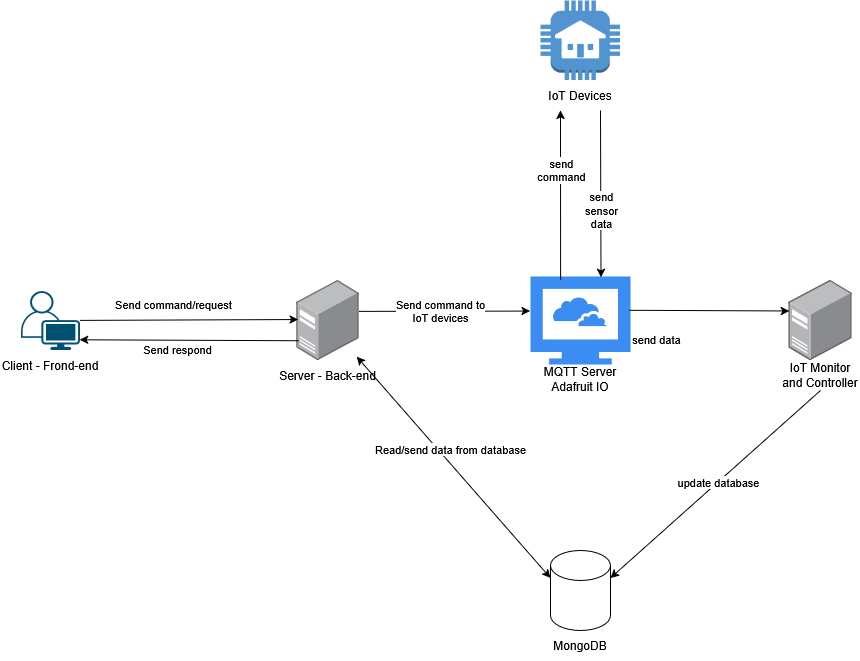
\includegraphics[width=1\linewidth]{content/images/SystemComponents.png}
    \caption{Kiến trúc tổng thể của hệ thống Green Sense}
    \label{fig:overallStructure}
\end{figure}

\textbf{Các thành phần chính}:
\begin{itemize}
\item \textit{Frontend (React)}: Cung cấp giao diện người dùng trực quan để giám sát trạng thái nhà kính, điều khiển thiết bị, và tương tác với tính năng điều khiển thiết bị bằng ngôn ngữ tự nhiên qua AI. Frontend gửi các yêu cầu đến backend qua API REST để thực hiện các thao tác.

\item \textit{Backend (Flask)}: Xử lý logic nghiệp vụ, quản lý dữ liệu và tiếp nhận các lệnh từ frontend. Backend có trách nhiệm điều phối hoạt động của thiết bị IoT thông qua giao thức MQTT và kết nối với cơ sở dữ liệu MongoDB để lưu trữ trạng thái và lịch sử hoạt động của hệ thống.

\item \textit{Database (MongoDB)}: Lưu trữ thông tin về trạng thái hiện tại của các thiết bị, dữ liệu cảm biến thu thập được và lịch sử hoạt động để phục vụ cho việc giám sát, phân tích và báo cáo.

\item \textit{Thiết bị IoT (tích hợp trên Yolo:Bit)}: Thiết bị vật lý chịu trách nhiệm thu thập dữ liệu cảm biến như nhiệt độ, độ ẩm, ánh sáng và thực thi các lệnh điều khiển nhận được từ hệ thống. Thiết bị giao tiếp với backend thông qua giao thức MQTT trên nền tảng Adafruit IO. Firmware của thiết bị được phát triển bằng ngôn ngữ C++ để đảm bảo hiệu suất và ổn định trong môi trường nhúng.

\item \textit{IoT Monitor and Controller (Python)}: Là module độc lập được phát triển bằng Python, có nhiệm vụ lắng nghe các dữ liệu cảm biến thời gian thực từ nền tảng Adafruit IO. Khi nhận dữ liệu, module này sẽ thực hiện việc bật/tắt các thiết bị nếu chế độ điều khiển đang được đặt ở trạng thái tự động. Đồng thời, nó sẽ lưu trữ dữ liệu thu thập được lên MongoDB để đảm bảo tính nhất quán và theo dõi trạng thái hệ thống.

\item \textit{Nền tảng MQTT – Adafruit IO}: Là dịch vụ trung gian đóng vai trò broker MQTT, kết nối backend và thiết bị IoT, đảm bảo việc truyền nhận dữ liệu và lệnh điều khiển được diễn ra một cách nhanh chóng, ổn định và theo thời gian thực.
\end{itemize}

\textbf{Luồng dữ liệu và tương tác giữa các thành phần}:
\begin{enumerate}
    \item Người dùng tương tác với giao diện frontend để thực hiện giám sát và điều khiển nhà kính.
    \item Frontend gửi yêu cầu thông qua API REST đến backend xử lý.
    \item Backend chuyển lệnh điều khiển đến thiết bị IoT qua giao thức MQTT trên Adafruit IO.
    \item Thiết bị IoT nhận lệnh và thực thi các hành động, đồng thời gửi dữ liệu cảm biến về lại Adafruit IO.
    \item Module IoT Monitor and Controller nhận dữ liệu cảm biến từ Adafruit IO, quyết định hành động bật/tắt thiết bị nếu ở chế độ tự động, và cập nhật dữ liệu vào MongoDB.
    \item Backend truy xuất dữ liệu từ MongoDB để phản hồi trạng thái và lịch sử hoạt động cho frontend hiển thị.
\end{enumerate}

\subsubsection{Thiết kế cơ sở dữ liệu}

Hệ thống sử dụng cơ sở dữ liệu để lưu trữ ba loại thông tin chính:
\begin{enumerate}
    \item Lịch sử hoạt động của các thiết bị IoT
    \item Dữ liệu thu thập từ các cảm biến (sensors)
    \item Thông tin về các tác vụ được người dùng cấu hình trong chế độ lập lịch hoạt động của thiết bị
\end{enumerate}

Do sử dụng MongoDB – một hệ quản trị cơ sở dữ liệu NoSQL dạng document – nên cấu trúc cơ sở dữ liệu không tuân theo mô hình quan hệ truyền thống. Thay vào đó, thiết kế được thể hiện dưới dạng Class Diagram, nhằm mô tả trực quan các trường dữ liệu có trong từng collection.

\begin{figure}[H]
    \centering
    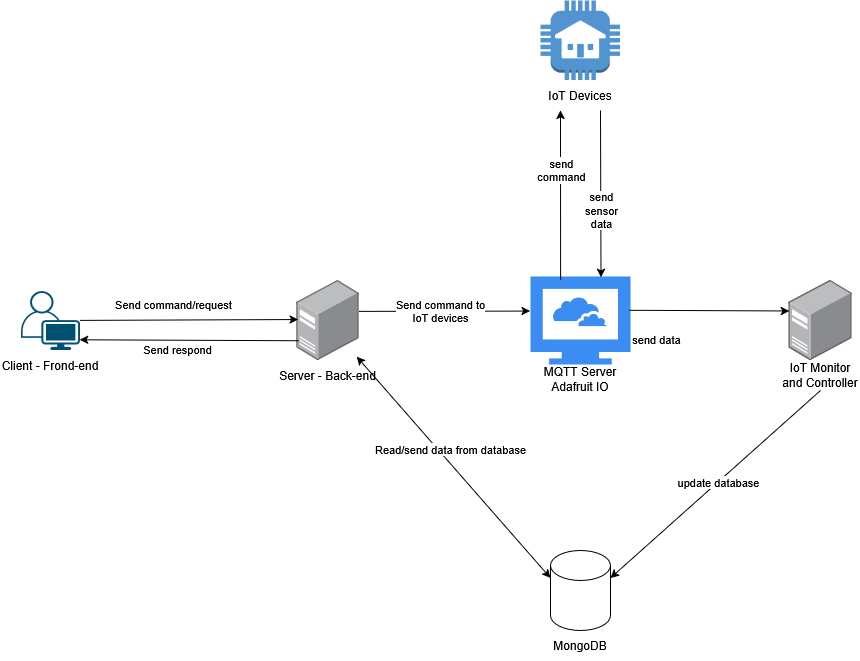
\includegraphics[width=1\linewidth]{content/images/SystemComponents.png}
    \caption{Class Diagram mô tả cấu trúc cơ sở dữ liệu MongoDB của hệ thống}
    \label{fig:classDiagram}
\end{figure}

Mô hình dữ liệu bao gồm các collection chính sau:
\begin{itemize}
    \item Activity: Lưu trữ các hoạt động của thiết bị với các thuộc tính gồm:
    \begin{itemize}
        \item \texttt{time} (datetime): Thời điểm ghi nhận hoạt động
        \item \texttt{data} (int): Giá trị định lượng của hoạt động
        \item \texttt{activity\_type} (str): Loại hoạt động được thực hiện
    \end{itemize}
    
    \item Humid, Light, Temperature: Mỗi collection lưu dữ liệu tương ứng từ cảm biến độ ẩm, ánh sáng và nhiệt độ. Các trường dữ liệu gồm:
    \begin{itemize}
        \item \texttt{time} (datetime): Thời điểm ghi nhận
        \item \texttt{data} (int): Giá trị đo được từ cảm biến
    \end{itemize}

    \item Scheduler\_job: Lưu thông tin về các job được người dùng lập lịch cho thiết bị. Các trường dữ liệu gồm:
    \begin{itemize}
        \item \texttt{job\_id} (str): Mã định danh của job
        \item \texttt{device\_id} (str): Mã thiết bị tương ứng
        \item \texttt{action} (str): Hành động sẽ được thực hiện
        \item \texttt{action\_options} (dict): Các tùy chọn cấu hình cho hành động
        \item \texttt{trigger} (str): Kiểu kích hoạt job (ví dụ: theo thời gian, sự kiện,...)
        \item \texttt{trigger\_options} (dict): Các tùy chọn cấu hình cho trigger
    \end{itemize}
\end{itemize}

Thiết kế này đảm bảo tính mở rộng, linh hoạt và dễ tích hợp với các hệ thống IoT, đồng thời phù hợp với đặc điểm lưu trữ phi quan hệ của MongoDB.

\newpage

